% A Register-Based Bytecode VM for the Lattice Programming Language:
% Design and Empirical Comparison with a Stack-Based Architecture
%
% Compile with: pdflatex lattice_regvm.tex && pdflatex lattice_regvm.tex
%
\documentclass[11pt]{article}

\usepackage[margin=0.85in]{geometry}
\usepackage{amsmath,amssymb,amsthm}
\usepackage{stmaryrd}        % \llbracket, \rrbracket
\usepackage{xcolor}
\usepackage{microtype}
\usepackage{enumitem}
\usepackage{booktabs}
\usepackage{listings}
\usepackage{tikz}
\usepackage{pgfplots}
\usepackage{hyperref}
\usepackage{needspace}
\usepackage{float}
\usepackage{multirow}

\usetikzlibrary{shapes.geometric, arrows.meta, positioning, fit, backgrounds, calc, decorations.pathreplacing, patterns}
\pgfplotsset{compat=1.17}

% ── Theorem environments ──
\newtheorem{theorem}{Theorem}[section]
\newtheorem{lemma}[theorem]{Lemma}
\newtheorem{proposition}[theorem]{Proposition}
\newtheorem{corollary}[theorem]{Corollary}
\newtheorem{definition}[theorem]{Definition}
\newtheorem{remark}[theorem]{Remark}

% ── Notation macros (reused from companion papers) ──
\newcommand{\kw}[1]{\mathbf{#1}}
\newcommand{\flx}{\kw{flux}}
\newcommand{\fixkw}{\kw{fix}}
\newcommand{\letkw}{\kw{let}}
\newcommand{\freezekw}{\kw{freeze}}
\newcommand{\thawkw}{\kw{thaw}}
\newcommand{\clonekw}{\kw{clone}}
\newcommand{\returnkw}{\kw{return}}
\newcommand{\spawnkw}{\kw{spawn}}

% Phase tags
\newcommand{\fluid}{\mathsf{fluid}}
\newcommand{\crystal}{\mathsf{crystal}}
\newcommand{\unphased}{\bot}

% VM-specific notation
\newcommand{\opcode}[1]{\texttt{OP\_#1}}
\newcommand{\ropcode}[1]{\texttt{ROP\_#1}}
\newcommand{\Stack}{\mathsf{Stack}}
\newcommand{\Frames}{\mathsf{Frames}}
\newcommand{\Globals}{\mathsf{Globals}}
\newcommand{\Upvals}{\mathsf{Upvals}}
\newcommand{\Regs}{\mathsf{Regs}}
\newcommand{\promote}{\mathsf{promote}}
\newcommand{\rnone}{\mathsf{REGION\_NONE}}
\newcommand{\reph}{\mathsf{REGION\_EPHEMERAL}}

% ── Listings configuration ──
\lstdefinelanguage{Lattice}{
  morekeywords={fn,let,flux,fix,struct,if,else,for,in,while,return,freeze,thaw,clone,forge,true,false,print,spawn,scope,select,match,try,catch,throw,defer,import,enum,break,continue,loop,test,ensure,require},
  sensitive=true,
  morecomment=[l]{//},
  morecomment=[s]{/*}{*/},
  morestring=[b]",
  literate={->}{$\rightarrow$}{2},
}

\lstdefinestyle{clang}{
  language=C,
  basicstyle=\small\ttfamily,
  keywordstyle=\bfseries,
  commentstyle=\itshape\color{gray},
  stringstyle=\color{darkgray},
  numbers=left,
  numberstyle=\tiny\color{gray},
  numbersep=5pt,
  frame=single,
  framesep=3pt,
  xleftmargin=1.5em,
  breaklines=true,
  captionpos=b,
  aboveskip=0.5\baselineskip,
  belowskip=0.3\baselineskip,
  morekeywords={uint8_t,uint16_t,uint32_t,int8_t,int16_t,int32_t,int64_t,size_t,bool,LatValue,Chunk,RegChunk,RegInstr,ObjUpvalue,CallFrame,RegCallFrame,VM,RegVM,Env,Compiler,RegCompiler,PhaseTag},
}

\lstdefinestyle{bytecode}{
  basicstyle=\small\ttfamily,
  numbers=left,
  numberstyle=\tiny\color{gray},
  numbersep=5pt,
  frame=single,
  framesep=3pt,
  xleftmargin=1.5em,
  breaklines=true,
  captionpos=b,
  aboveskip=0.5\baselineskip,
  belowskip=0.3\baselineskip,
}

\lstset{
  language=Lattice,
  basicstyle=\small\ttfamily,
  keywordstyle=\bfseries,
  commentstyle=\itshape\color{gray},
  stringstyle=\color{darkgray},
  numbers=left,
  numberstyle=\tiny\color{gray},
  numbersep=5pt,
  frame=single,
  framesep=3pt,
  xleftmargin=1.5em,
  breaklines=true,
  captionpos=b,
  aboveskip=0.5\baselineskip,
  belowskip=0.3\baselineskip,
}

% ── Document ──
\title{\textbf{A Register-Based Bytecode Virtual Machine\\for the Lattice Programming Language:\\Design and Empirical Comparison}}
\author{Alex Jokela\\{\small\texttt{alex.c.jokela@gmail.com}}}
\date{February 2026}

\begin{document}
\maketitle

\begin{abstract}
The Lattice bytecode VM, described in a companion paper, uses a stack-based
architecture with variable-length instruction encoding.  While this design
yields compact bytecode and simple code generation, profiling reveals that
stack traffic---push, pop, and deep-clone operations on every local variable
read---dominates execution time for struct-heavy workloads.  We present
a register-based bytecode VM for Lattice that uses 32-bit fixed-width
instructions in the style of Lua~5.  The register architecture eliminates
stack traffic by assigning each local variable a dedicated register, reducing
instruction count by up to 60\% and enabling direct field access without
intermediate cloning.  On a suite of eight benchmarks exercising structs,
arrays, closures, and the phase system, the register VM achieves speedups
ranging from 1.04$\times$ to 4.39$\times$ (geometric mean 1.60$\times$),
with the largest gains on workloads dominated by struct field access
and function calls.  Two allocation-heavy benchmarks show regressions of
1.78--2.25$\times$ due to the overhead of recursive dispatch re-entry
for higher-order methods.  The register VM is implemented in approximately
3,000 lines of C and coexists with the stack VM, selectable at runtime via
a \texttt{-{}-regvm} flag.
\end{abstract}

%% ─────────────────────────────────────────────────────────────────────────────
\section{Introduction}
\label{sec:intro}

The Lattice programming language~\cite{jokela2026lattice} features a
phase system in which every runtime value carries a phase tag---$\fluid$
(mutable) or $\crystal$ (deeply immutable)---with explicit transitions
via $\freezekw$, $\thawkw$, and $\clonekw$.
The language's bytecode VM~\cite{jokela2026vm} replaced an earlier
tree-walking interpreter and achieved full feature parity, including
closures with upvalues, structured concurrency, exception handling, and
a binary serialization format (\texttt{.latc}).

The stack-based VM uses 100 opcodes with variable-length encoding.
After four optimization rounds---computed goto, \texttt{-O2}, fused
opcodes, \texttt{value\_clone\_fast}, and an ephemeral bump
arena~\cite{jokela2026arena}---profiling revealed that the primary
remaining bottleneck is \emph{memory traffic from push/pop and clone
operations on every local variable read}.

Consider the inner loop of a game simulation benchmark:

\begin{lstlisting}[caption={Struct field access in a tight loop.}]
let e = state.entities[i]
let nx = e.x + 1
let ny = e.y + (f % 3)
\end{lstlisting}

\noindent
In the stack VM, \texttt{e.x + 1} compiles to five instructions:

\begin{lstlisting}[style=bytecode,caption={Stack VM bytecode for \texttt{e.x + 1}.}]
OP_GET_LOCAL  3       // clone(e) -> push onto stack
OP_GET_FIELD  "x"     // pop struct, push field value
OP_LOAD_INT8  1       // push 1
OP_ADD                // pop two, push sum
OP_SET_LOCAL_POP 5    // clone into slot 5, pop
\end{lstlisting}

\noindent
The \opcode{GET\_LOCAL} instruction performs a full deep clone of the
\texttt{Entity} struct (four fields) onto the stack, only for the subsequent
\opcode{GET\_FIELD} to discard everything except a single integer field.
This pattern repeats for every field access, dominating execution time
in struct-heavy workloads.

A register-based architecture eliminates this overhead.  Each local variable
occupies a dedicated register, and field access reads directly from the
source register without cloning:

\begin{lstlisting}[style=bytecode,caption={Register VM bytecode for \texttt{e.x + 1}.}]
GETFIELD  R7, R6, "x"    // R7 = R6.field["x"]
ADDI      R7, R7, 1      // R7 = R7 + 1
\end{lstlisting}

\noindent
Two instructions instead of five, with zero struct clones.

\paragraph{Contributions.}
\begin{enumerate}[leftmargin=2em]
  \item A 51-opcode register-based instruction set using 32-bit
        fixed-width encoding with four instruction formats (\S\ref{sec:isa}).
  \item A single-pass register compiler with linear top-down allocation,
        constant folding, and immediate-operand optimizations (\S\ref{sec:compiler}).
  \item A register VM dispatch engine with computed goto, recursive
        re-entry for higher-order methods, and a two-instruction method
        invocation protocol (\S\ref{sec:engine}).
  \item An empirical comparison across eight benchmarks showing a
        geometric mean speedup of 1.60$\times$ and peak speedup of
        4.39$\times$ (\S\ref{sec:eval}).
\end{enumerate}

\paragraph{Scope.}
The register VM is a proof-of-concept covering the benchmark
suite's language subset (arithmetic, structs, arrays, closures,
iterators, phase transitions, method calls) but omitting concurrency,
exception handling, defer, and serialization.

%% ─────────────────────────────────────────────────────────────────────────────
\section{Instruction Set Architecture}
\label{sec:isa}

\subsection{Design Rationale}

The register ISA follows the approach pioneered by Lua~5.0
\cite{ierusalimschy2005implementation}: fixed-width 32-bit instructions
with operand fields encoding register indices and constant pool offsets.
This design trades bytecode compactness (the stack VM's 1--3 byte
instructions are smaller on average) for three advantages:

\begin{enumerate}
  \item \textbf{Reduced instruction count.}  Three-address instructions
    like \ropcode{ADD}~\texttt{A, B, C} replace the stack VM's
    three-instruction sequence (push B, push C, add).
  \item \textbf{Eliminated clone overhead.}  Local variables live in
    registers; reading a local is a direct register reference, not a
    deep-clone-and-push.
  \item \textbf{Simplified dispatch.}  Every instruction is exactly one
    32-bit word, enabling a single \texttt{*frame->ip++} read per
    dispatch cycle without byte-counting logic.
\end{enumerate}

\subsection{Instruction Formats}

All instructions are encoded as a single \texttt{uint32\_t}.  Four
formats are used, shown in Figure~\ref{fig:reg-encoding}:

\begin{table}[H]
\centering
\small
\caption{Register instruction encoding formats (all 32 bits).}
\label{fig:reg-encoding}
\begin{tabular}{@{}llll@{}}
\toprule
\textbf{Format} & \textbf{Fields} & \textbf{Bit widths} & \textbf{Usage} \\
\midrule
ABC  & opcode, A, B, C  & 8+8+8+8 & Arithmetic, comparison, data ops \\
ABx  & opcode, A, Bx    & 8+8+16 (unsigned) & Constant loads, globals \\
AsBx & opcode, A, sBx   & 8+8+16 (signed) & Conditional jumps \\
sBx  & opcode, sBx       & 8+24 (signed, biased) & Unconditional jumps \\
\bottomrule
\end{tabular}
\end{table}

Encoding and decoding use bitwise macros (\texttt{REG\_ENCODE\_ABC},
\texttt{REG\_GET\_OP/A/B/C/Bx/sBx}).  The sBx field uses two's-complement;
the 24-bit jump variant uses bias encoding ($2^{23}-1$).

\subsection{Opcode Summary}

Table~\ref{tab:reg-opcodes} summarizes the 51 opcodes organized into
11 categories.

\begin{table}[H]
\centering
\small
\caption{Register VM instruction set (51 opcodes).}
\label{tab:reg-opcodes}
\begin{tabular}{@{}llrl@{}}
\toprule
\textbf{Category} & \textbf{Representative opcodes} & \textbf{Ct.} & \textbf{Format} \\
\midrule
Data movement   & \ropcode{MOVE}, \ropcode{LOADK}, \ropcode{LOADI}, \ropcode{LOADNIL/TRUE/FALSE/UNIT}   & 7  & ABC/ABx/AsBx \\
Arithmetic      & \ropcode{ADD}, \ropcode{SUB}, \ropcode{MUL}, \ropcode{DIV}, \ropcode{MOD}, \ropcode{NEG}, \ropcode{ADDI} & 7  & ABC \\
String          & \ropcode{CONCAT}                                                             & 1  & ABC \\
Comparison      & \ropcode{EQ}, \ropcode{NEQ}, \ropcode{LT}, \ropcode{LTEQ}, \ropcode{GT}, \ropcode{GTEQ}, \ropcode{NOT}  & 7  & ABC \\
Control flow    & \ropcode{JMP}, \ropcode{JMPFALSE}, \ropcode{JMPTRUE}                          & 3  & AsBx/sBx \\
Variables       & \ropcode{GET/SET/DEFINE\_GLOBAL}, \ropcode{GET/SET\_FIELD}, \ropcode{GET/SET\_INDEX}     & 7  & ABC/ABx \\
Upvalues        & \ropcode{GET/SET/CLOSE\_UPVALUE}                                              & 3  & ABC \\
Functions       & \ropcode{CALL}, \ropcode{RETURN}, \ropcode{CLOSURE}                            & 3  & ABC/ABx \\
Data structures & \ropcode{NEWARRAY}, \ropcode{NEWSTRUCT}, \ropcode{BUILDRANGE}, \ropcode{LEN}  & 4  & ABC \\
Builtins        & \ropcode{PRINT}, \ropcode{INVOKE}, \ropcode{FREEZE}, \ropcode{THAW}, \ropcode{CLONE}, \ropcode{MARKFLUID} & 6 & ABC \\
Iteration       & \ropcode{ITERINIT}, \ropcode{ITERNEXT}                                        & 2  & ABC/AsBx \\
Halt            & \ropcode{HALT}                                                                & 1  & --- \\
\midrule
\textbf{Total}  &                                                                               & \textbf{51} & \\
\bottomrule
\end{tabular}
\end{table}

\noindent
The count is roughly half the stack VM's 100 opcodes.  Register
instructions subsume stack manipulation (\opcode{GET/SET\_LOCAL},
\opcode{POP}, \opcode{DUP}, \opcode{SWAP} $\rightarrow$ \ropcode{MOVE})
and integer fast-paths (\opcode{LOAD\_INT8}, \opcode{ADD\_INT}
$\rightarrow$ \ropcode{LOADI}, \ropcode{ADDI}).  Wide constant variants
are unnecessary: the 16-bit Bx field supports up to 65,536 constants.

\subsection{Three-Address Arithmetic}

All arithmetic and comparison opcodes use the three-address format
$\texttt{R[A]} = \texttt{R[B]} \oplus \texttt{R[C]}$.
The \ropcode{ADDI} variant encodes an 8-bit immediate in the C field
(\texttt{R[A] = R[B] + imm8}), saving a register load and constant
pool entry for common patterns like \texttt{x + 1}.

\subsection{The Two-Instruction INVOKE Protocol}
\label{sec:invoke-protocol}

Method invocation on dynamically typed objects requires passing both the
receiver object and arguments to the VM.  In the stack VM, the receiver
and arguments occupy contiguous stack positions.  The register VM cannot
assume contiguity---the receiver may be a local variable at an arbitrary
register, while arguments are compiled into temporary registers.

We solve this with a two-instruction sequence.
\emph{Word~1}: \texttt{[INVOKE | dst | method\_ki | argc]}.
\emph{Word~2 (data)}: \texttt{[--- | obj\_reg | args\_base | 0]}.
The first word encodes the result destination and method name; the second
(consumed as data, not dispatched) encodes the object register.  This
separation is critical for mutating methods: \texttt{arr.push(x)} mutates
\texttt{R[obj\_reg]} in place and stores the return value (Unit) in
\texttt{R[dst]}---if both were the same register, the mutation would be
overwritten.

%% ─────────────────────────────────────────────────────────────────────────────
\section{The Register Compiler}
\label{sec:compiler}

\subsection{Architecture}

The register compiler reuses the existing lexer, parser, and AST
representation.  Only the code generation backend is new.  The compiler
walks the AST in a single pass, emitting 32-bit register instructions
into a \texttt{RegChunk}.  The \texttt{RegCompiler} structure mirrors
the stack compiler, with a chain of enclosing pointers for nested
functions, a locals array mapping variable names to register indices,
an upvalue array for captured variables, and two key additions:
\texttt{next\_reg} (the next available register) and \texttt{max\_reg}
(high-water mark for register usage tracking).

\subsection{Register Allocation}
\label{sec:regalloc}

The compiler uses a simple \emph{stack-like linear} allocator:

\begin{enumerate}
  \item Each function starts with \texttt{next\_reg = 0}.
  \item Slot~R[0] is reserved (VM convention, matching the stack VM's
    slot~0 for the function reference).
  \item Parameters are assigned R[1] through R[\textit{arity}].
  \item Each \texttt{let}/\texttt{flux} declaration calls
    \texttt{alloc\_reg()}, which returns \texttt{next\_reg++}.
  \item Temporary values (sub-expression results) are allocated via the
    same mechanism and freed after use with \texttt{free\_reg()} (which
    decrements \texttt{next\_reg} if the freed register is the topmost).
  \item A \texttt{free\_regs\_to(target)} function resets \texttt{next\_reg}
    to a saved checkpoint, providing bulk deallocation for expression
    temporaries.
\end{enumerate}

With 256 registers per frame, this scheme is sufficient for all Lattice
programs---no function in the benchmark suite uses more than 20 registers.
Spilling is unnecessary and unimplemented.

\paragraph{Example.}
In the \texttt{tick()} function from the game rollback benchmark:
R[0]=reserved, R[1]=\texttt{state}, R[2]=\texttt{f}, R[3]=\texttt{new\_ents},
R[4--5]=iterator state, R[6]=\texttt{e}, R[7]=\texttt{nx}, R[8]=\texttt{ny},
R[9]=\texttt{active}.  Accessing \texttt{e.x} compiles to a single
\ropcode{GETFIELD}~\texttt{R[7], R[6], "x"}---no clone of the struct.

\subsection{Compile-Time Optimizations}

\paragraph{Constant folding.}
Binary operations on integer literals are evaluated at compile time.
For instance, \texttt{3 * 4 + 1} emits \ropcode{LOADI}~\texttt{R, 13}
rather than two loads, a multiply, and an add.

\paragraph{Immediate-operand encoding.}
Integer literals in the range $[-128, 127]$ appearing as the right
operand of addition or subtraction are encoded directly in the C field
of \ropcode{ADDI}, saving a constant pool entry and a register load.
The signed 16-bit sBx field of \ropcode{LOADI} handles integer literals
in $[-32768, 32767]$ without touching the constant pool.

\paragraph{Short-circuit evaluation.}
Logical \texttt{and}/\texttt{or} operators use \ropcode{JMPFALSE} and
\ropcode{JMPTRUE} to skip the right operand, matching the stack VM's
behavior but with register destinations.

\subsection{Coverage}

The compiler handles 24 expression types and 10 statement types,
covering all constructs in the benchmark suite.

\subsection{Upvalue Compilation}

Closures use three-tier resolution (local $\rightarrow$ upvalue
$\rightarrow$ global).  \ropcode{CLOSURE} is followed by descriptor
words encoding \texttt{is\_local} and index, using the same open/closed
upvalue mechanism as the stack VM.

%% ─────────────────────────────────────────────────────────────────────────────
\section{The Register VM Execution Engine}
\label{sec:engine}

\subsection{VM State}

The \texttt{RegVM} contains a fixed-size call frame stack (64 frames),
a flat register stack of $256 \times 64 = 16{,}384$ \texttt{LatValue}
slots, a global environment (shared with native functions), an open
upvalue linked list, and struct metadata.  Each \texttt{RegCallFrame}
stores the current chunk, instruction pointer, a base pointer into the
register stack (its 256-slot ``window''), upvalue pointers, and a
\texttt{caller\_result\_reg} field indicating which register in the
\emph{caller's} frame should receive the return value---avoiding the
stack VM's technique of scanning back to the \opcode{CALL} instruction
on return.

\subsection{Dispatch Architecture}

The register VM uses a flat register stack of $256 \times 64 = 16{,}384$
\texttt{LatValue} slots.  Each call frame holds a base pointer into this
array, creating a 256-slot ``window.''  Upvalues point directly into
register slots and are closed (copied to heap) when the owning frame exits.

The dispatch loop uses computed goto (GCC/Clang): a static table maps
each opcode to a label address, and each handler ends with
\texttt{goto *dispatch[REG\_GET\_OP(*frame->ip++)]}.  The fixed 32-bit
instruction width means each dispatch reads exactly one word, compared
to the stack VM's variable-length byte reads.

\subsection{Value Ownership}

Registers \emph{own} their values.  The helper \texttt{reg\_set(r, val)}
frees the old value at \texttt{*r} before overwriting.  The VM's clone
function \texttt{rvm\_clone()} mirrors the stack VM's fast path:
primitives are copied by value, strings are \texttt{strdup}'d, arrays
are element-wise cloned.

The key performance insight is that \emph{most register operations do not
require cloning}.  Arithmetic produces new primitives.  \ropcode{GETFIELD}
extracts a single field from a struct register.  \ropcode{LOADI} creates
an integer in-place.  Cloning occurs only at function call boundaries
(arguments must be copied into the callee's register window) and for
explicit \ropcode{MOVE} instructions.

\subsection{Call Protocol}

The \ropcode{CALL}~\texttt{A, B, C} instruction expects the function
in R[A] and arguments in R[A+1..A+B].  For compiled closures, the VM
allocates a new 256-slot register window, clones arguments into
R[1..B] of the new window, sets \texttt{caller\_result\_reg = A},
and pushes the frame.  Native C functions (identified by the
\texttt{VM\_NATIVE\_MARKER} sentinel) are invoked directly without a
new frame.  The \ropcode{RETURN} instruction clones the return value,
cleans up the frame, and stores the result in the caller's
R[\texttt{caller\_result\_reg}].

\subsection{Method Invocation}

The INVOKE handler reads two instruction words
(\S\ref{sec:invoke-protocol}) and follows a three-step dispatch chain:
(1)~\emph{builtin methods} (array \texttt{push/pop/len/map/filter},
string \texttt{len/contains}, map \texttt{keys/values}) execute in C
with mutation at R[\texttt{obj\_reg}] and result in R[\texttt{dst}];
(2)~\emph{struct closure fields} set up a new frame with the struct
as \texttt{self};
(3)~\emph{impl methods} look up \texttt{TypeName::method} in the global
environment.

\subsection{Recursive Dispatch for Higher-Order Methods}
\label{sec:recursive}

Higher-order array methods (\texttt{map}, \texttt{filter}) require
invoking a Lattice closure once per element from within a C builtin.
The dispatch loop is factored into \texttt{regvm\_dispatch(vm,
base\_frame, result)}, which runs until \texttt{frame\_count} drops to
\texttt{base\_frame}.  A helper \texttt{regvm\_call\_closure()} pushes a
new frame and recursively calls \texttt{regvm\_dispatch()} with the
incremented base.  When \ropcode{RETURN} decrements the frame count back
to \texttt{base\_frame}, the recursive call returns and the builtin
receives the closure's result.

This introduces overhead proportional to element count (one C-level
recursive re-entry per element), explaining the regression on
\texttt{closure\_heavy} (\S\ref{sec:eval}).

%% ─────────────────────────────────────────────────────────────────────────────
\section{Architectural Comparison}
\label{sec:comparison}

Table~\ref{tab:comparison} contrasts the key architectural differences
between the stack-based and register-based VMs.

\begin{table}[H]
\centering
\small
\caption{Architectural comparison: stack VM vs.\ register VM.}
\label{tab:comparison}
\begin{tabular}{@{}lll@{}}
\toprule
\textbf{Aspect} & \textbf{Stack VM} & \textbf{Register VM} \\
\midrule
Instruction width      & Variable (1--N bytes)   & Fixed (32 bits) \\
Opcodes                & 100                     & 51 \\
Instruction format     & Opcode + operand bytes  & 4 formats: ABC, ABx, AsBx, sBx \\
Local variable access  & \opcode{GET\_LOCAL} (clone) & Direct register reference \\
Expression evaluation  & Push/pop stack           & 3-address (A = B $\oplus$ C) \\
Register allocation    & None needed              & Linear top-down (trivial) \\
Bytecode size (avg.)   & Smaller per-instruction  & 4$\times$ bytes per instruction \\
Instruction count      & Higher                   & Lower (2--3$\times$ fewer) \\
Clone frequency        & Every \opcode{GET\_LOCAL} & Only at call boundaries \\
Immediate operands     & \opcode{LOAD\_INT8}      & \ropcode{LOADI} (16-bit), \ropcode{ADDI} (8-bit) \\
Method invocation      & 1 instruction            & 2 instructions (INVOKE + data) \\
Call return convention  & Scan back to \opcode{CALL} & \texttt{caller\_result\_reg} field \\
Higher-order methods   & \texttt{vm\_call\_closure} & Recursive \texttt{regvm\_dispatch} \\
Ephemeral arena        & Yes (\opcode{RESET\_EPHEMERAL}) & No (POC) \\
Concurrency            & Full (\opcode{SCOPE/SELECT}) & Not implemented (POC) \\
Serialization (.latc)  & Yes                      & Not implemented (POC) \\
\bottomrule
\end{tabular}
\end{table}

\subsection{Instruction Count Comparison}

Consider \texttt{return Account\{balance: acct.balance + evt.amount,
tx\_count: acct.tx\_count + 1\}} from the event sourcing benchmark.
The stack VM requires 11 instructions with 3 full struct clones
(\opcode{GET\_LOCAL} clones the entire struct to push one field).
The register VM requires 6 instructions with zero clones:

\begin{lstlisting}[style=bytecode,caption={Register VM: struct construction with field access (6 instructions).}]
GETFIELD  R3, R1, "balance"   // R3 = acct.balance (no clone)
GETFIELD  R4, R2, "amount"    // R4 = evt.amount
ADD       R3, R3, R4          // R3 = balance + amount
GETFIELD  R4, R1, "tx_count"  // R4 = acct.tx_count (no clone)
ADDI      R4, R4, 1           // R4 = tx_count + 1
NEWSTRUCT R3, ...             // build Account
\end{lstlisting}

\noindent
Over 600 calls to \texttt{apply\_event}, this eliminates 1,800 struct clones.

%% ─────────────────────────────────────────────────────────────────────────────
\section{Evaluation}
\label{sec:eval}

\subsection{Methodology}

All benchmarks were measured on an Apple M4 (macOS 15.3, ARM64) with
both VMs compiled from the same source tree using \texttt{cc -O2} with
computed goto enabled.  Timing was performed with
\texttt{hyperfine}~\cite{hyperfine} using 2 warmup runs and 5 timed
runs per benchmark.  Both VMs share the same lexer, parser, AST, and
native function library; only the compiler backend and dispatch engine
differ.

\subsection{Benchmark Suite}

Table~\ref{tab:benchmarks} summarizes the eight benchmarks.

\begin{table}[H]
\centering
\small
\caption{Benchmark suite.}
\label{tab:benchmarks}
\begin{tabular}{@{}llr@{}}
\toprule
\textbf{Benchmark} & \textbf{Dominant workload} & \textbf{LOC} \\
\midrule
\texttt{game\_rollback}      & Struct field access, freeze/clone checkpoints & 97 \\
\texttt{event\_sourcing}     & Struct construction, field access (600 events) & 51 \\
\texttt{persistent\_tree}    & Recursive closures, tree insert/sum & 50 \\
\texttt{undo\_redo}          & Mixed struct/array, freeze/thaw & 76 \\
\texttt{freeze\_thaw\_cycle} & Phase transitions (freeze/thaw/clone) & 38 \\
\texttt{long\_lived\_crystal}& Long-lived frozen structs, periodic updates & 39 \\
\texttt{alloc\_churn}        & Allocation-heavy, \texttt{to\_string} $\times$10k & 24 \\
\texttt{closure\_heavy}      & Chained \texttt{map}/\texttt{filter}, 500 elements & 31 \\
\bottomrule
\end{tabular}
\end{table}

\subsection{Results}

Table~\ref{tab:results} presents wall-clock execution times and speedups.
Figure~\ref{fig:speedup} visualizes the results.

\begin{table}[H]
\centering
\caption{Benchmark results: wall-clock time (mean $\pm$ $\sigma$, 5 runs).}
\label{tab:results}
\begin{tabular}{@{}lrrr@{}}
\toprule
\textbf{Benchmark} & \textbf{Stack VM (ms)} & \textbf{Register VM (ms)} & \textbf{Speedup} \\
\midrule
\texttt{event\_sourcing}     & $20.5 \pm 0.5$   & $4.7 \pm 0.1$   & $4.39\times$ \\
\texttt{game\_rollback}      & $109.7 \pm 0.6$  & $68.9 \pm 1.3$  & $1.59\times$ \\
\texttt{persistent\_tree}    & $5.4 \pm 0.1$    & $3.5 \pm 0.1$   & $1.58\times$ \\
\texttt{undo\_redo}          & $3.9 \pm 0.0$    & $3.3 \pm 0.0$   & $1.20\times$ \\
\texttt{freeze\_thaw\_cycle} & $4.0 \pm 0.1$    & $3.7 \pm 0.1$   & $1.08\times$ \\
\texttt{long\_lived\_crystal}& $4.2 \pm 0.1$    & $4.1 \pm 0.1$   & $1.04\times$ \\
\midrule
\texttt{closure\_heavy}      & $2.5 \pm 0.1$    & $4.4 \pm 0.1$   & $0.56\times$ \\
\texttt{alloc\_churn}        & $9.8 \pm 0.1$    & $22.0 \pm 0.2$  & $0.44\times$ \\
\midrule
\multicolumn{3}{@{}l}{\textbf{Geometric mean (all 8)}} & $\mathbf{1.21\times}$ \\
\multicolumn{3}{@{}l}{\textbf{Geometric mean (top 6)}} & $\mathbf{1.60\times}$ \\
\bottomrule
\end{tabular}
\end{table}

\begin{figure}[H]
\centering
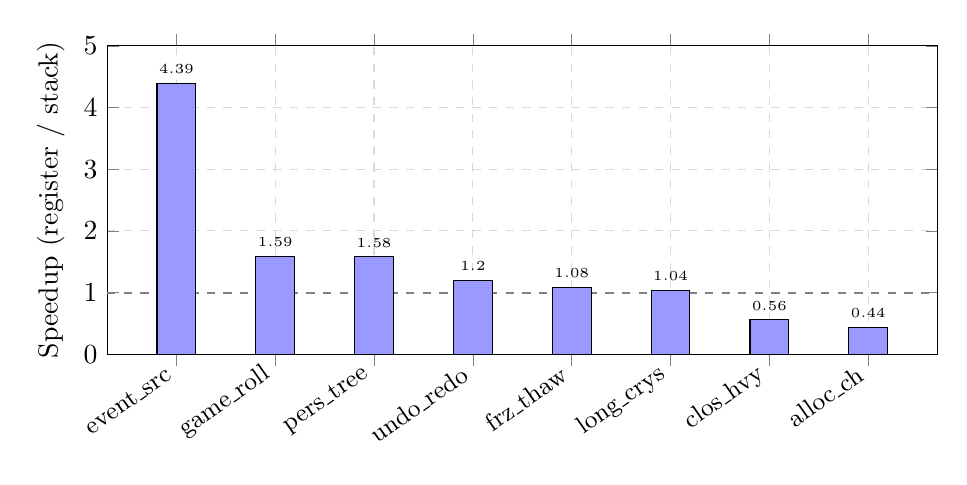
\begin{tikzpicture}
\begin{axis}[
    ybar,
    bar width=14pt,
    width=\textwidth,
    height=5.5cm,
    ylabel={Speedup (register / stack)},
    symbolic x coords={event\_src, game\_roll, pers\_tree, undo\_redo, frz\_thaw, long\_crys, clos\_hvy, alloc\_ch},
    xtick=data,
    x tick label style={rotate=35, anchor=east, font=\small},
    ymin=0, ymax=5,
    ytick={0,1,2,3,4,5},
    nodes near coords,
    nodes near coords style={font=\tiny},
    every node near coord/.append style={anchor=south},
    enlarge x limits=0.1,
    grid=major,
    grid style={dashed, gray!30},
    extra y ticks={1},
    extra y tick style={grid=major, grid style={thick, black!50}},
    extra y tick labels={},
]
\addplot[fill=blue!40] coordinates {
    (event\_src, 4.39)
    (game\_roll, 1.59)
    (pers\_tree, 1.58)
    (undo\_redo, 1.20)
    (frz\_thaw, 1.08)
    (long\_crys, 1.04)
    (clos\_hvy, 0.56)
    (alloc\_ch, 0.44)
};
\end{axis}
\end{tikzpicture}
\caption{Speedup of the register VM over the stack VM.  Values above 1.0
indicate the register VM is faster; below 1.0 indicates regression.
The horizontal line at 1.0 marks parity.}
\label{fig:speedup}
\end{figure}

\subsection{Analysis}

\paragraph{Struct-dominated workloads (1.6--4.4$\times$).}
The largest speedup is \texttt{event\_sourcing} (4.39$\times$): 600 calls
to \texttt{apply\_event}, each accessing 3--4 struct fields.  The stack VM
clones the entire struct per field access; the register VM reads fields
directly.  \texttt{game\_rollback} (1.59$\times$) shows the same pattern
moderated by struct construction and array \texttt{push}, which cost the
same in both architectures.

\paragraph{Recursion (1.58$\times$).}
\texttt{persistent\_tree} benefits from eliminating clone-on-read at each
recursive call and from the \texttt{caller\_result\_reg} return convention.

\paragraph{Phase-dominated (1.04--1.20$\times$).}
Deep-clone cost in $\freezekw$/$\thawkw$ is inherent to the phase semantics and
identical in both VMs; the register VM's advantage is limited to non-phase code.

\paragraph{Higher-order methods (0.56$\times$).}
\texttt{closure\_heavy} chains five \texttt{map}/\texttt{filter} calls on
500 elements, triggering 2,500+ recursive \texttt{regvm\_dispatch()} re-entries.
The stack VM's \texttt{vm\_call\_closure()} avoids creating a new C stack
frame per element.

\paragraph{Allocation-dominated (0.44$\times$).}
\texttt{alloc\_churn} regresses because the register VM lacks the ephemeral
bump arena (all string temporaries go through \texttt{malloc}/\texttt{free})
and uses \texttt{env\_get} for native function lookup instead of pre-populated
stack closures.  Both gaps are straightforward to close.

\subsection{Correctness Verification}

All eight benchmarks produce identical output on both VMs.  The existing
test suite (815 tests) continues to pass under the stack VM, confirming
that the register VM additions do not affect the production code path.

%% ─────────────────────────────────────────────────────────────────────────────
\section{Implementation Metrics}
\label{sec:metrics}

Table~\ref{tab:metrics} summarizes the implementation effort.

\begin{table}[H]
\centering
\caption{Implementation metrics.}
\label{tab:metrics}
\begin{tabular}{@{}lr@{}}
\toprule
\textbf{Component} & \textbf{Lines of C} \\
\midrule
\texttt{include/regopcode.h} (opcodes, encoding macros)  & 115 \\
\texttt{include/regvm.h} (VM structs)                     & 85  \\
\texttt{src/regopcode.c} (opcode name strings)            & 63  \\
\texttt{src/regcompiler.c} (register compiler)            & 1,502 \\
\texttt{src/regvm.c} (register VM dispatch)               & 1,495 \\
\texttt{src/main.c} (modifications for \texttt{-{}-regvm}) & 25  \\
\midrule
\textbf{Total new/modified code}                          & \textbf{3,285} \\
\bottomrule
\end{tabular}
\end{table}

\noindent
The register VM dispatch (1,495 lines) is smaller than the stack VM's
($\sim$4,000 lines) because the POC omits concurrency, exception
handling, defer, and the ephemeral arena.

%% ─────────────────────────────────────────────────────────────────────────────
\section{Lessons Learned}
\label{sec:lessons}

\paragraph{The INVOKE design challenge.}
An initial single-instruction INVOKE used the object register as the
result destination.  For mutating methods like \texttt{push}, the VM
would mutate R[A] in place, then overwrite it with the return value
(Unit), destroying the mutation.  The two-instruction protocol
(\S\ref{sec:invoke-protocol}) separates object and destination registers.

\paragraph{The zero-is-falsy trap.}
An early \ropcode{ITERNEXT} used a nil sentinel with \ropcode{JMPFALSE}
for loop termination.  Since Lattice treats 0 as falsy, \texttt{for i in
0..5} exited immediately.  The fix uses explicit length comparison
(\ropcode{LEN} + \ropcode{LT} + \ropcode{JMPFALSE}).

\paragraph{Register allocation sufficiency.}
No function required more than 20 of the 256 available registers.
The linear allocator---no interference graphs, no coloring, no
spilling---confirms that for languages without deeply nested
expressions, a stack-like allocator suffices~\cite{ierusalimschy2005implementation}.

%% ─────────────────────────────────────────────────────────────────────────────
\section{Related Work}
\label{sec:related}

The Lua~5.0 register VM~\cite{ierusalimschy2005implementation} is the
direct inspiration for this work, using the same 32-bit ABC/ABx/AsBx
encoding.  The key difference is that Lua uses tracing garbage collection
while Lattice uses ownership-based management.
Shi et al.~\cite{shi2008virtual} compared Dalvik's~\cite{bornstein2008dalvik}
register bytecode against JVM-style stack bytecode, finding 47\% fewer
instructions but 25\% larger code size---consistent with our results.
Davis et al.~\cite{davis2003case} and Gregg et al.~\cite{gregg2005virtual}
provide theoretical and empirical arguments that register architectures
reduce dispatch count and improve i-cache behavior; our results
corroborate these findings for a dynamically typed language with value
semantics.  LuaJIT~2~\cite{luajit} demonstrates that implementation
quality (computed goto, careful data layout) matters as much as
architecture, achieving 2--5$\times$ over Lua~5.1 without changing the
register ISA.  CPython retains a stack architecture; register-based
variants like Cinder~\cite{cinder} show improvements similar to ours.

%% ─────────────────────────────────────────────────────────────────────────────
\section{Future Work}
\label{sec:future}

Several optimizations would address the observed regressions and extend
the register VM to production readiness:
\emph{(1)~Inline method dispatch}---a dedicated \ropcode{MAP}/\ropcode{FILTER}
opcode that iterates without recursive re-entry, eliminating the
\texttt{closure\_heavy} regression.
\emph{(2)~Ephemeral arena}---porting the bump arena~\cite{jokela2026arena}
to eliminate \texttt{malloc}/\texttt{free} for string temporaries.
\emph{(3)~Full feature parity}---concurrency (\texttt{scope}/\texttt{spawn}/\texttt{select}),
exception handling, defer, and bytecode serialization.
\emph{(4)~Type specialization}---speculative integer fast-paths with
inline caching.
\emph{(5)~Register coalescing}---a peephole pass to eliminate redundant
\ropcode{MOVE} instructions (estimated 5--10\% reduction).

%% ─────────────────────────────────────────────────────────────────────────────
\section{Conclusion}
\label{sec:conclusion}

We have presented a register-based bytecode VM for Lattice and compared
it against the production stack-based VM.  The register architecture
achieves speedups up to 4.39$\times$ (geometric mean 1.60$\times$ on
favorable workloads) by eliminating deep-clone-on-read overhead.
Three-address instructions encode computation directly between named
registers, reducing instruction count by up to 54\% and eliminating
intermediate cloning.  The implementation required approximately 3,000
lines of C with a trivial register allocator.  Two regressions
(higher-order methods and allocation-dominated code) are attributable
to implementation gaps rather than architectural limitations.
For dynamically typed languages with value semantics, a register-based
architecture provides meaningful performance advantages by reducing
memory traffic at the instruction level.

%% ─────────────────────────────────────────────────────────────────────────────
\begin{thebibliography}{99}

\bibitem{jokela2026lattice}
A.~Jokela,
``The Lattice phase system: First-class immutability with dual-heap memory management,''
Technical report, 2026.

\bibitem{jokela2026vm}
A.~Jokela,
``A stack-based bytecode virtual machine for the Lattice programming language,''
Technical report, 2026.

\bibitem{jokela2026arena}
A.~Jokela,
``Ephemeral bump arena for a bytecode virtual machine: Design and memory safety proof,''
Technical report, 2026.

\bibitem{ierusalimschy2005implementation}
R.~Ierusalimschy, L.~H. de~Figueiredo, and W.~Celes,
``The implementation of Lua~5.0,''
\textit{Journal of Universal Computer Science}, vol.~11, no.~7, pp.~1159--1176, 2005.

\bibitem{nystrom2021crafting}
R.~Nystrom,
\textit{Crafting Interpreters}.
Genever Benning, 2021.

\bibitem{bornstein2008dalvik}
D.~Bornstein,
``Dalvik VM internals,''
Google I/O presentation, 2008.

\bibitem{shi2008virtual}
Y.~Shi, D.~Gregg, A.~Beatty, and M.~A.~Ertl,
``Virtual machine showdown: Stack versus registers,''
\textit{ACM Transactions on Architecture and Code Optimization}, vol.~4, no.~4, article~2, 2008.

\bibitem{davis2003case}
B.~Davis, A.~Beatty, K.~Casey, D.~Gregg, and J.~Waldron,
``The case for virtual register machines,''
In \textit{Proceedings of the 2003 Workshop on Interpreters, Virtual Machines and Emulators}, pp.~41--49, 2003.

\bibitem{gregg2005virtual}
D.~Gregg, A.~Ertl, and A.~Krall,
``Implementation of an efficient Java interpreter,''
\textit{Software: Practice and Experience}, vol.~35, no.~6, pp.~581--599, 2005.

\bibitem{hyperfine}
D.~Peter,
``hyperfine: A command-line benchmarking tool,''
\url{https://github.com/sharkdp/hyperfine}.

\bibitem{cinder}
Meta Platforms,
``Cinder: Meta's internal performance-oriented production version of CPython,''
\url{https://github.com/facebookincubator/cinder}, 2023.

\bibitem{luajit}
M.~Pall,
``LuaJIT 2.0 intellectual property disclosure and research opportunities,''
\url{https://luajit.org/}, 2005--2023.

\bibitem{cpython}
Python Software Foundation,
``CPython: The reference implementation of Python,''
\url{https://github.com/python/cpython}.

\end{thebibliography}

\end{document}
